\addcontentsline{toc}{chapter}{Samenvatting}

\begin{otherlanguage}{dutch}
\sisetup{output-decimal-marker={,}}
\pgfkeys{/pgf/number format/.cd, use comma}

\chapter*{Samenvatting}
\setcounter{equation}{0}
\setcounter{figure}{0}
\ihead{Samenvatting}

Het onderzoeksgebied der deeltjesfysica bestudeert de kleinste bouwstenen waaruit het universum is opgebouwd: elementaire deeltjes.
De grootte van deze deeltjes is vele malen kleiner dan alles wat we in het dagelijks leven tegenkomen, zelfs vele malen kleiner dan cellen.
De drie elementaire deeltjes waaruit atomen bestaan -- en waar wij dus uiteindelijk allemaal uit bestaan -- zijn \emph{up} en \emph{down} quarks, en elektronen.

In de eerste helft van de vorige eeuw is een interessant fenomeen ontdekt: antimaterie.
Antimateriedeeltjes gedragen zich precies hetzelfde als gewone materie, op twee dingen na: hun lading is tegengesteld, en ze komen maar heel beperkt voor in de natuur.
Vooral dat laatste is interessant voor fundamenteel onderzoek.
Wanneer materie in grote deeltjesversnellers geproduceerd wordt, wordt er altijd exact evenveel antimaterie geproduceerd.
Als we nu terug in de tijd gaan, tot de oerknal, zou ons universum uit exact even veel materie als antimaterie moeten bestaan!

Maar dat is niet het geval.
Wij, onze planeet, het zonnestelsel en alle sterren en hemellichamen die we kunnen waarnemen bestaan uit materie.
Dus is de grote vraag: waar is alle antimaterie heen?
Het onderzoek in dit proefschrift hoopt bij te dragen aan een antwoord op deze fundamentele vraag.

\begin{figure}[htb] \centerfloat
    \begin{tikzpicture}
        \node[anchor=south west,inner sep=0] (image) at (0,0) {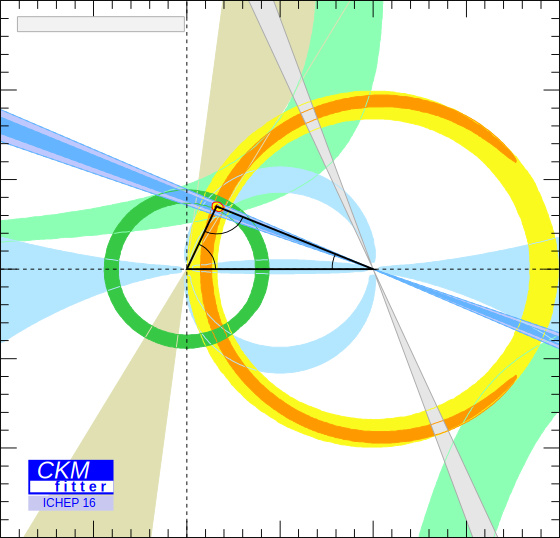
\includegraphics[width=0.55\textwidth]{theory/rhoeta_large}};
        \begin{scope}[x={(image.south east)},y={(image.north west)}]
            \node at (1. / 6. - 0.02, -0.027) {\(\pgfmathprintnumber[fixed,precision=1,fixed zerofill=true]{-0.5}\)};
            \foreach \x in {0, 2, 3, ..., 6}
            {
                \tikzmath{\xpos = \x / 6.; \xtext = \x * 0.5 - 1.0;}
                \node at (\xpos, -0.027) {\(\pgfmathprintnumber[fixed,precision=1,fixed zerofill=true]{\xtext}\)};
            }
            \node[anchor=east] at (0.005, 0.008) {\(\pgfmathprintnumber[fixed,precision=1,fixed zerofill=true]{-1.5}\)};
            \foreach \y in {1, ..., 6}
            {
                \tikzmath{\ypos = \y / 6.; \ytext = \y * 0.5 - 1.5;}
                \node[anchor=east] at (0.005, \ypos) {\(\pgfmathprintnumber[fixed,precision=1,fixed zerofill=true]{\ytext}\)};
            }

            {
                \fontsize{4}{4.8}\selectfont
                \node[anchor=west] at (0.04, 0.955) {excluded area has \({\text{CL} > \num{0.95}}\)};
                \node[anchor=west,rotate=-68] at (0.475, 0.995) {excluded at \({\text{CL} > \num{0.95}}\)};
                \node[anchor=west] at (0.76, 0.08) {sol. w/ \({\cos 2\CPbeta < 0}\)};
                \node[anchor=west] at (0.76, 0.05) {(excl. at \({\text{CL} > \num{0.95}}\))};
            }
            {
                \fontsize{10}{12}\selectfont
                \node[anchor=west] at (0.40, 0.885) {\CPgamma};
                \node[anchor=west] at (0.665, 0.810) {\dmd~\&~\dms};
                \node[anchor=west] at (0.02, 0.730) {\({\sin 2\CPbeta}\)};
                \node[anchor=west] at (0.82, 0.630) {\dmd};
                \node[anchor=west] at (0.03, 0.575) {\epsK};
            }
            {
                \fontsize{7}{8.4}\selectfont
                \node[anchor=west] at (0.365, 0.580) {\CPalpha};
                \node[anchor=west] at (0.530, 0.519) {\CPbeta};
                \node[anchor=west] at (0.34, 0.514) {\CPgamma};
            }
            {
                \fontsize{10}{12}\selectfont
                \node[anchor=west] at (0.03, 0.460) {\CPalpha};
                \node[anchor=west] at (0.175, 0.390) {\abs{\Vub}};
                \node[anchor=west] at (0.59, 0.390) {\CPalpha};
                \node[anchor=west] at (0.205, 0.165) {\CPgamma};
                \node[anchor=west] at (0.86, 0.190) {\epsK};
            }

            \node[anchor=east] at (1.0, -0.10) {\wolfrhob};
            \node[rotate=90,anchor=east,inner xsep=0pt,outer xsep=0pt] at (-0.12, 1.0) {\wolfetab};
        \end{scope}
    \end{tikzpicture}
    \caption{
        Een van de zogeheten \emph{unitariteitsdriehoeken} van het Standaard~Model.
        De oppervlakte van de driehoek is een maat voor de hoeveelheid \CP-schending die in de natuur voorkomt.
        De gekleurde gebieden representeren ieder een andere meting van \CP-schending, en de grootte van het gebied de onzekerheid van die meting.
        De apex van de driehoek ligt binnen de onzekerheid van al die metingen, wat een sterk argument is voor de validiteit van het model.
        Het onderzoek in dit proefschrift betreft de parameter~\CPgamma, in de linkeronderhoek van de driehoek.
        Over deze parameter is relatief weinig bekend, zoals ook te zien is aan het grote gekleurde gebied, dat de onzekerheid aangeeft.}
    \label{fig:samenvatting_UT}
\end{figure}
%
Een mogelijke uitleg is dat materie en antimaterie zich heel vergelijkbaar gedragen, maar net niet helemaal hetzelfde.
De schending van de symmetrie tussen materie en antimaterie wordt \CP-schending genoemd.
Een kleine hoeveelheid \CP-schending wordt voorspeld door onze huidige fysische kennis (zie \cref{fig:samenvatting_UT}).
De hoeveelheid \CP-schending die we in de natuur zien is echter bij lange na niet voldoende om het verschil tussen de hoeveelheid materie en antimaterie te verklaren.
Vooralsnog blijft het daarom een open vraag: wat is er met de antimaterie gebeurd?

\begin{figure}[htb] \centerfloat
    \hspace*{-.5cm}
    \begin{tikzpicture}[font=\captionfont]
        \node[anchor=south west,inner sep=0] (image) at (0,0) {\includegraphics[width=1.\textwidth]{detector/LHCb}};
        \begin{scope}[x={(image.south east)},y={(image.north west)}]
            \draw [very thick, ->] (-.1, .45) -- (.01, .45) node [at start,anchor=north west] {\normalsize \proton};
            \draw [very thick, ->] (.95, .45) -- (.84, .45) node [at start,anchor=north east] {\normalsize \proton};

            \draw [very thick] (.11, .47) -- (.11, 0.85) node [right,anchor=north west,inner ysep=0pt,outer sep=0pt] {\velo};
            \draw [very thick] (.16, .54) -- (.16, 0.80) node [right,anchor=north west,inner ysep=0pt,outer sep=0pt] {\rich~1};
            \draw [very thick] (.185,.48) -- (.185,0.75) node [right,anchor=north west,inner ysep=0pt,outer sep=0pt] {\ttracker};
            \draw [very thick] (.27, .65) -- (.27, 0.85) node [right,anchor=north west,inner ysep=0pt,outer sep=0pt] {Magneet};
            \draw [very thick] (.413,.57) -- (.413,0.85) node [right,anchor=north west,inner ysep=0pt,outer sep=0pt] {\intr~\&~\ot};
            \draw [very thick] (.46, .61) -- (.46, 0.78) node [right,anchor=north west,inner ysep=0pt,outer sep=0pt] {\rich~2};
            \draw [very thick] (.57, .61) -- (.57, 0.85) node [right,anchor=north west,inner ysep=0pt,outer sep=0pt] {\presh~\&~\ecal};
            \draw [very thick] (.62, .63) -- (.62, 0.78) node [right,anchor=north west,inner ysep=0pt,outer sep=0pt] {\hcal};
            \draw [very thick] (.75, .67) -- (.75, 0.85) node [right,anchor=north west,inner ysep=0pt,outer sep=0pt,align=left] {Muon-\\stations};
        \end{scope}
    \end{tikzpicture}
    \caption{
        Doorsnede van de \lhcb-detector.
        De onderdelen van de detector zijn aangegeven in de figuur.
        De protonen van de~\lhc botsen links in de figuur, binnenin de~\velo.}
    \label{fig:samenvatting_LHCb}
\end{figure}
%
Het onderzoek in dit proefschrift hoopt meer inzicht te verschaffen in \CP-schending in het verval van vreemde schoonheidsmesonen: \Bs-mesonen, en hun antideeltjes \Bsb-mesonen.
Deze deeltjes kunnen niet direct worden waargenomen, maar alleen door middel van de deeltjes waarin ze na korte tijd vanzelf uiteen vallen: hun vervalsproducten.
In dit proefschrift wordt gekeken naar het verval van een \Bs-meson naar twee vervalsproducten: een \Dsmp-meson en een kaon~(\Kpm).
Deze deeltjes kunnen worden waargenomen door een deeltjesdetector, in dit geval de \lhcb-detector (zie \cref{fig:samenvatting_LHCb}) bij de Large Hadron Collider van~\cern, in Gen\`eve.
Deze detector is de grootte van een huis, en bevindt zich \SI{80}{\metre}~onder het aardoppervlak.
In de detector botsen protonen van de~\lhc tegen elkaar, nadat ze versneld zijn tot meer dan~\SI{99.999}{\percent} van de lichtsnelheid.
Deze botsingen generen enorme hoeveelheden deeltjes, waaronder \Bs-mesonen.

Allereerst is onderzocht hoe vaak dit specifieke verval van \Bs-mesonen voorkomt in verhouding tot alle andere mogelijke vervallen van zulke deeltjes: de vervalsverhouding.
Dit getal kan worden berekend met behulp van het aantal waargenomen \BsDsK-vervallen en de effici\"entie waarmee deze kunnen worden gemeten.
Die effici\"entie kan worden bepaald door middel van simulaties, waarin de volledige proton-protoninteracties, vervallen, materiaalinteracties en detectorrespons accuraat worden gesimuleerd.
De waargenomen vervalsverhouding is ongeveer~\num{2} promille, wat een totaal geeft van rond de \num{5000}~\BsDsK-vervallen in de data.
De grote piek aan linkerkant van \cref{fig:samenvatting_mass} bevat deze vervallen.

Uit deze vervallen kan \CP-schending worden gemeten dankzij een interessante eigenschap van \Bs-mesonen: gedurende hun (korte) leven veranderen ze met hoge frequentie in hun overeenkomstige antideeltje en weer terug.
Dit fenomeen heet \emph{vermenging} en kan slechts gebeuren in enkele soorten deeltjes.
\CP-schending kan voorkomen als asymmetrie tussen twee vergelijkbare processen: het vermengen en vervallen van een meson, en het vermengen en vervallen van het overeenkomstige antimeson.
Hierdoor kan \CP-schending worden gemeten door het bestuderen van het verval van \Bs-mesonen.

Om vermenging goed waar te kunnen nemen is het noodzakelijk te weten hoe lang een meson leefde voordat het verviel.
Deze levensduur kan worden bepaald met behulp van de massa en impuls van het meson:
%
\begin{equation} \tag{1} \label{eqn:samenvatting_resolution}
    t = \dfrac{m \upDelta x}{\ptot} \rlap{,}
\end{equation}
%
met \(t\)~de levensduur van het meson, \(m\)~zijn massa, \(\upDelta x\)~de afgelegde afstand, en \(\ptot\)~de impuls.
Dit getal kan alleen worden gebruikt in combinatie met de onzekerheid erop.
Een eerste schatting van deze onzekerheid kan worden berekend uit de onzekerheden op de getallen aan de rechterkant van \cref{eqn:samenvatting_resolution}.
Het is echter bekend dat deze schatting de daadwerkelijke onzekerheid onderschat.
Daarom dient deze te worden gekalibreerd.%
%
\begin{figure}[tb] \centerfloat
    \begin{tikzpicture}[scale=0.7, every node/.style={scale=0.7}]
        \node[anchor=south west,inner sep=0] (image) at (0,0) {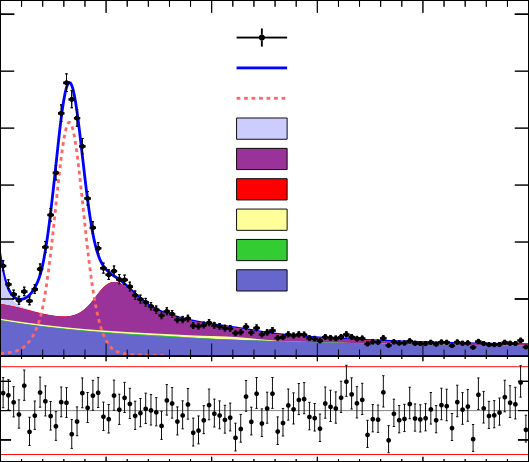
\includegraphics[width=0.9\textwidth]{BsDsK_TD/MDFit_Results/mass_Bs2DsK_BeautyMass_both_all_run1_nominal}};
        \begin{scope}[x={(image.south east)},y={(image.north west)}]
            \foreach \x/\xtext in {5300, 5400, ..., 5800}
            {
                \tikzmath{\xpos = (\x - 5300) / (5800 - 5300);}
                \node at (\xpos, -0.025) {\(\xtext\)};
            }
            \foreach \y in {0, ..., 6}
            {
                \tikzmath{\ypos = (\y / 6) * 0.740 + 0.217; \ytext = 200 * \y;}
                \node[anchor=base east] at (0.005, \ypos) {\(\pgfmathprintnumber[fixed,precision=0,fixed zerofill=true,1000 sep={}]{\ytext}\)};
            }
            \foreach \p in {0, ..., 2}
            {
                \tikzmath{\ypos = (\p / 2) * 0.127 + .048; \ptext = (\p - 1) * 2;}
                \node[anchor=east] at (0.005, \ypos) {\(\scriptstyle\pgfmathprintnumber[fixed,precision=0,fixed zerofill=true]{\ptext}\)};
            }
            \node[anchor=east] at (1.0, -0.09) {\({m(\DsmpKpm)}~[\si{\MeVcc}]\)};
            \node[rotate=90,anchor=east,inner xsep=0pt,outer xsep=0pt] at (-0.11, 1.0) {\({\text{Kandidaten}/(\SI{5.0}{\MeVcc})}\)};
            \node[anchor=west] at (0.06, 0.92) {\Huge\lhcb};
            % Legend
            {
                \node[anchor=base west] at (0.55, 0.906) {Data};
                \node[anchor=base west] at (0.55, 0.906 - 1 * 0.0656) {Totale fit};
                \node[anchor=base west] at (0.55, 0.906 - 2 * 0.0656) {\BsDsK~(signaal)};
                \node[anchor=base west] at (0.55, 0.906 - 3 * 0.0656) {\decay{\BorBsz}{\DsorDssmp\KorKstpm}};
                \node[anchor=base west] at (0.55, 0.906 - 4 * 0.0656) {\decay{\Bs}{\DsorDssm(\pip, \rhop)}};
                \node[anchor=base west] at (0.55, 0.906 - 5 * 0.0656) {\decay{\Bd}{\Dm(\pip, \Kp)}};
                \node[anchor=base west] at (0.55, 0.906 - 6 * 0.0656) {\LbDsOrDsstp};
                \node[anchor=base west] at (0.55, 0.906 - 7 * 0.0656) {\decay{\Lb}{\Lcp(\pim, \Km)}};
                \node[anchor=base west] at (0.55, 0.906 - 8 * 0.0656) {Combinatoriek};
            }
        \end{scope}
    \end{tikzpicture}
    \caption{
        Verdeling van de invariante massa van de combinatie van \Dsmp- en \Kpm-mesonen, zoals bepaald in het onderzoek dat in dit proefschrift wordt beschreven.
        De onderbroken lijn aan de linkerkant van de figuur geeft de massa van het \Bs-meson aan (ongeveer~\SI{5367}{\MeVcc}), en de piek in de data op die plek geeft aan dat de juiste vervallen aanwezig zijn.
        De gekleurde gebieden zijn achtergronddata, en dragen niet bij aan de meting.}
    \label{fig:samenvatting_mass}
\end{figure}
%
\begin{figure}[tb] \centerfloat
    \begin{tikzpicture}[scale=0.7, every node/.style={scale=0.7}]
        \node[anchor=south west,inner sep=0] (image) at (0,0) {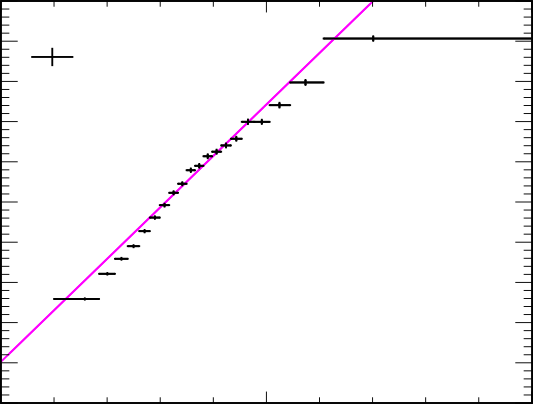
\includegraphics[width=0.9\textwidth]{summary/CombinationLinear_ALL_eff_sigma}};
        \begin{scope}[x={(image.south east)},y={(image.north west)}]
            \foreach \x in {0, ..., 10}
            {
                \tikzmath{\xpos = (\x / 10); \xtext = 10 * \x;}
                \node at (\xpos, -0.025) {\(\pgfmathprintnumber[fixed,precision=0,fixed zerofill=true]{\xtext}\)};
            }
            \foreach \y in {0, ..., 10}
            {
                \tikzmath{\ypos = (\y / 10); \ytext = 10 * \y;}
                \node[anchor=east] at (0.005, \ypos) {\(\pgfmathprintnumber[fixed,precision=0,fixed zerofill=true]{\ytext}\)};
            }
            % Legend
            {
                \node[anchor=base west] at (0.14, 0.843) {Prompte~\Dspm-data};
            }
            \node[anchor=east] at (1.0, -0.09) {Oorspronkelijke schatting van de onzekerheid~\([\si{\fs}]\)};
            \node[rotate=90,anchor=east,inner xsep=0pt,outer xsep=0pt] at (-0.12, 1.0) {Gekalibreerde onzekerheid op de levensduur~\({\sigma~[\si{\fs}]}\)};
        \end{scope}
    \end{tikzpicture}
    \caption{
        Onzekerheid op de levensduur, gemeten met prompte \Dsmp-vervallen (zwarte datapunten), als functie van de oorspronkelijke schatting van de onzekerheid.
        De lijn is een lineaire fit aan deze data.
        De gradi\"ent van deze lijn is de schaalfactor tussen de oorspronkelijk schatting en de daadwerkelijke onzekerheid op de levensduur, en is ongeveer~\num{1.3}.}
    \label{fig:samenvatting_resolution}
\end{figure}
%
Deze kalibratie moet worden uitgevoerd met vervallen waarvan de levensduur al bekend is.
In dit geval zijn dat direct vervallen, of prompte, \Dsmp-vervallen.
Ieder prompt \Dsmp-meson is gecombineerd met een kaon, zodanig dat er een ``nep''-\Bs-meson ontstaat: het lijkt op een echte, maar door het prompte verval is de levensduur gelijk aan nul.
Hierom kan vanuit de spreiding van de waargenomen levensduur de daadwerkelijke onzekerheid op de levensduur bepaald worden.
Door dit te vergelijken met de eerdere schatting voor de onzekerheid kan een schaalfactor bepaald worden, zoals weergegeven in \cref{fig:samenvatting_resolution}.
Deze schaalfactor kan op de echte \Bs-vervallen worden toegepast om de onzekerheden te kalibreren.

Met de vervalstijden en gekalibreerde onzekerheid op die getallen kan de \CP-schending in de data gemeten worden.
Hiervoor moeten de mesonen voorzien worden van een \emph{tag}, die aangeeft of ze geproduceerd zijn als een \Bs-meson of als de tegenhanger, een \Bsb-meson.
Zo ontstaan er vier vervalscombinaties: een \Bs- of \Bsb-meson, die beide kunnen vervallen naar een van beide eindtoestanden~\DsmKp of~\DspKm.
Door deze vier combinaties te analyseren kunnen vijf \CP-schendingsparameters bepaald worden: \Cpar, \Spar, \Sbpar, \Dpar, en~\Dbpar.
Samen leiden deze parameters tot een meting van de parameter~\CPgamma (ge\"introduceerd in \cref{fig:samenvatting_UT}), zoals ge\"illustreerd in \cref{fig:samenvatting_gamma}.

Het resultaat is~\({\CPgamma = \ang[parse-numbers=false]{\left(128_{-22}^{+17}\right)}}\), wat significant afwijkt van \ang[parse-numbers=false]{\left(0\!\mod 180\right)} en daarom het eerste bewijs voor \CP-schending is in het verval~\BsDsK.
De waarde is ongeveer \num{2.3}~standaarddeviaties hoger dan verwacht uit eerdere metingen van \lhcb:~\({\CPgamma = \ang[parse-numbers=false]{\left(72.2_{-7.3}^{+6.8}\right)}}\).
Deze afwijking is klein genoeg dat het een statistische fluctuatie zou kunnen zijn.
Desalniettemin zou het een indicatie voor nieuwe fysica kunnen zijn, zoals een verschil in \CP-schending voor \Bp-mesonvervallen, die voornamelijk zijn gebruikt voor het \lhcb-resultaat, en \Bs-mesonvervallen waarop het onderzoek in dit proefschrift is gebaseerd.
%
\begin{figure}[htb] \centerfloat
    \fontsize{18}{21.6}\selectfont
    \begin{tikzpicture}[scale=0.8, every node/.style={scale=0.8}]
        \node[anchor=south west,inner sep=0] (image) at (0,0) {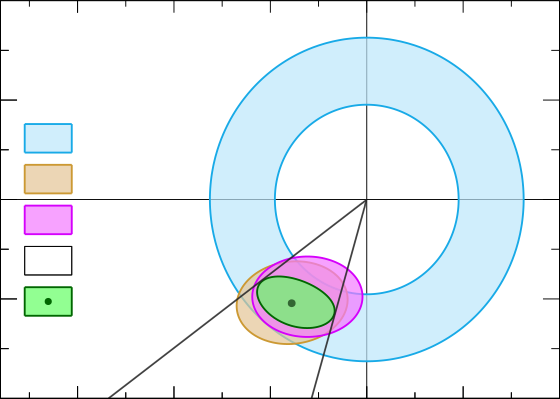
\includegraphics[width=0.9\textwidth]{Vub/Gamma/Lambda_f}};
        \begin{scope}[x={(image.south east)},y={(image.north west)}]
            \node at (0.139 + 0 * 0.172 - 0.02, -0.040) {\num{-1.5}};
            \node at (0.139 + 1 * 0.172 - 0.02, -0.040) {\num{-1}};
            \node at (0.139 + 2 * 0.172 - 0.02, -0.040) {\num{-0.5}};
            \node at (0.139 + 3 * 0.172, -0.040) {\num{0}};
            \node at (0.139 + 4 * 0.172, -0.040) {\num{0.5}};
            \node at (1.0, -0.040) {\num{1}};
            \node[anchor=east] at (0.005, 0.00) {\num{-1}};
            \node[anchor=east] at (0.005, 0.25) {\num{-0.5}};
            \node[anchor=east] at (0.005, 0.50) {\num{ 0}};
            \node[anchor=east] at (0.005, 0.75) {\num{ 0.5}};
            \node[anchor=east] at (0.005, 1.00) {\num{ 1}};

            % Legend
            {
                \fontsize{12}{14.4}\selectfont
                \node[anchor=base west] at (0.130, 0.640) {\(\sqrt{1 - \Cpar^{2}}\)};
                \node[anchor=base west] at (0.130, 0.640 - 1 * 0.103) {\({(-\Dpar, \Spar)}\)};
                \node[anchor=base west] at (0.130, 0.640 - 2 * 0.103) {\({(-\Dbpar, \Sbpar)}\)};
                \node[anchor=base west] at (0.130, 0.640 - 3 * 0.103) {\({-\left(\weak\right)}\)};
                \node[anchor=base west] at (0.130, 0.640 - 4 * 0.103) {Combinatie};
            }

            \node[anchor=east] at (1.0, -0.155) {\({\Im\left[2\lf / (1 + \abs{\lf}^{2})\right]}\)};
            \node[rotate=90,anchor=east,inner xsep=0pt,outer xsep=0pt] at (-0.14, 1.0) {\({\Re\left[2\lf / (1 + \abs{\lf}^{2})\right]}\)};
            \node[anchor=base west] at (0.06, 0.823) {\lhcb};
        \end{scope}
    \end{tikzpicture}
    \caption{
        De waarde van~\CPgamma die door de in dit proefschrift gepresenteerde analyse is bepaald~(zwarte lijnen en groen gekleurd gebied) en de waarden van de vijf \CP-schendingsparameters waardoor dit tot stand is gekomen~(andere gekleurde gebieden).
        De hoek tussen de combinatie en het punt~\({(0, 1)}\) geeft een waarde~\({\CPgamma = \ang[parse-numbers=false]{\left(\num{72.2}_{\num{-7.3}}^{+\num{6.8}}\right)}}\).}
    \label{fig:samenvatting_gamma}
\end{figure}

\sisetup{output-decimal-marker={.}}
\end{otherlanguage}

